\documentclass[11pt, dvipsnames, handout]{beamer}
\newtoggle{full}
\settoggle{full}{true}

\newtoggle{covered}
\settoggle{covered}{false}

\newtoggle{presentable}
\settoggle{presentable}{false}

\newtoggle{dualscreen}
\settoggle{dualscreen}{false}

\usepackage{pgfplots}
%\pgfplotsset{compat = newest}

\usepackage{pgfpages}

\setbeamertemplate{note page}{\pagecolor{yellow!5}\vfill \insertnote \vfill}
\usepackage{collect}
\definecollection{notes}
\newcounter{notestaken}

\usepackage{xpatch}

\usepackage{ulem}

\usepackage[framemethod=tikz]{mdframed}

\usepackage{scalerel}
\usepackage{calc}

%\usepackage{enumitem}
\setlength\fboxsep{.2em}

\usepackage{graphicx} % Allows including images
\usepackage{booktabs} % Allows the use of \toprule, \midrule and \bottomrule in tables

\xpatchcmd{\itemize}
  {\def\makelabel}
  {\setlength{\itemsep}{0.65 em}\def\makelabel}
  {}
  {}


\xpatchcmd{\beamer@enum@}
  {\def\makelabel}
  {\setlength{\itemsep}{0.65 em}\def\makelabel}
  {}
  {}


%\makeatletter
%\renewcommand{\itemize}[1][]{%
%  \beamer@ifempty{#1}{}{\def\beamer@defaultospec{#1}}%
%  \ifnum \@itemdepth >2\relax\@toodeep\else
%    \advance\@itemdepth\@ne
%    \beamer@computepref\@itemdepth% sets \beameritemnestingprefix
%    \usebeamerfont{itemize/enumerate \beameritemnestingprefix body}%
%    \usebeamercolor[fg]{itemize/enumerate \beameritemnestingprefix body}%
%    \usebeamertemplate{itemize/enumerate \beameritemnestingprefix body begin}%
%    \list
%      {\usebeamertemplate{itemize \beameritemnestingprefix item}}
%      {%
%        \setlength\topsep{1em}%NEW
%        \setlength\partopsep{1em}%NEW
%        \setlength\itemsep{1em}%NEW
%        \def\makelabel##1{%
%          {%
%            \hss\llap{{%
%                \usebeamerfont*{itemize \beameritemnestingprefix item}%
%                \usebeamercolor[fg]{itemize \beameritemnestingprefix item}##1}}%
%          }%
%        }%
%      }
%  \fi%
%  \beamer@cramped%
%  \raggedright%
%  \beamer@firstlineitemizeunskip%
%}
%
%
%
%
%
%\makeatother

%\setlist[beamer@enum@]{topsep=1 em}
%\let\origcheckmark\checkmark %screw you dingbat
%\let\checkmark\undefined %screw you dingbat
%\usepackage{dingbat} 
%\let\checkmark\origcheckmark %screw you dingbat






%\usepackage{fontawesome}

\usepackage{mathtools}
\usepackage{etoolbox, calculator}

\usepackage{xcolor}
\usepackage{tikz}
\usetikzlibrary{arrows.meta}
\usetikzlibrary{calc}
\usepackage[nomessages]{fp}
\usepackage{transparent}
\usepackage{accsupp}
%\usepackage{color, xcolor}

%colorblind-friendly palette
%\definecolor{dblue}{RGB}{51,34,136}
\definecolor{lblue}{RGB}{136,204,238}
%\definecolor{green}{RGB}{17,119,51}
\definecolor{tan}{RGB}{221,204,119}
%\definecolor{mauve}{RGB}{204,102,119}

\usepackage{tcolorbox}



\usepackage{xifthen}
\usepackage{nicefrac}
\usepackage{amsmath}
\usepackage{amsthm}
\usepackage{amssymb}
\theoremstyle{definition}
\newtheorem*{define}{Definition}
\newtheorem*{recall}{Recall}


\DeclareMathOperator{\tr}{tr}

\usepackage{multicol}
%\setlength{\columnsep}{1cm}

\usepackage{tablists, amsmath,vwcol, cancel, polynom}
\usetikzlibrary{shapes, patterns, decorations.shapes}
%\usepackage{tikzpeople}
\tikzstyle{vertex}=[shape=circle, minimum size=2mm, inner sep=0, fill]
\tikzstyle{opendot}=[shape=circle, minimum size=2mm, inner sep=0, fill=white, draw]

% common math quick commands
\newcommand{\nicedd}[2]{\nicefrac{\text{d}#1}{\text{d}#2}}
\newcommand{\dd}[2]{\dfrac{\text{d}#1}{\text{d}#2}}
\newcommand{\pd}[2]{\dfrac{\partial #1}{\partial#2}}
\renewcommand{\d}[1]{\text{d}#1}
\newcommand{\ddn}[3]{\dfrac{\text{d}^{#3}#1}{\text{d}#2^{#3}}}
\newcommand{\pdn}[3]{\dfrac{\partial^{#3}#1}{\partial#2^{#3}}}
\newcommand{\p}[0]{^{\prime}}
\newcommand{\pp}[0]{^{\prime\prime}}
\newcommand{\op}[2][\text{L}]{#1 \left[ #2 \right]}

\newcommand{\lap}[1]{\mathcal{L}\left\{#1\right\}}
\newcommand{\lapinv}[1]{\mathcal{L}^{-1}\left\{#1\right\}}
\newcommand{\lapint}[1]{\int_0^\infty e^{-st}#1dt}
\newcommand{\evalat}[2]{\Big|_{#1}^{#2}}

\newcommand{\paren}[1]{ \left( #1 \right)}

\newcommand{\haxis}[4][\normcolor]{\draw[#1, <->] (-#2,0)--(#3,0) node[right]{$#4$}; }


\newcommand{\axis}[4]{\draw[\normcolor, <->] (-#1,0)--(#2,0) 
node[right]{$x$};
\draw[help lines, <->] (0,-#3)--(0,#4) node[above]{$y$};}

\newcommand{\laxis}[6]{\draw[<->] (-#1,0)--(#2,0) 
node[right]{$#5$};
\draw[ <->] (0,-#3)--(0,#4) node[above]{$#6$};}
\newcommand{\xcoord}[2]{
	\draw (#1,.2)--(#1,-.2) node[below]{$#2$};}
\newcommand{\textnode}[3]{
	\draw (#1,#2) node[below]{$#3$};}
	
\newcommand{\nxcoord}[2]{
	\draw (#1,-.2)--(#1,.2) node[above]{$#2$};}
\newcommand{\ycoord}[2]{
	\draw (.2,#1)--(-.2,#1) node[left]{$#2$};}
\newcommand{\nycoord}[2]{
	\draw (-.2,#1)--(.2,#1) node[right]{$#2$};}
\newcommand{\dlim}{\displaystyle\lim}
\newcommand{\dlimx}[1]{\displaystyle\lim_{x \rightarrow #1}}
\newcommand{\stickfig}[2]{
	\draw (#1,#2) arc(-90:270:2mm);
	\draw (#1,#2)--(#1,#2-.5) (#1-.25,#2-.75)--(#1,#2-.5)--(#1+.25,#2-.75) (#1-.2,#2-.2)--(#1+.2,#2-.2);}	

%\newcounter{example}
%\setcounter{example}{1}
%\newcounter{preFrameExample}
%\AtBeginEnvironment{frame}{\setcounter{preFrameExample}{\value{example}}}
%\newcommand{\ex}[1]{
%	 \setcounter{example}{\value{preFrameExample}}
%	 \textcolor{green}{\small\fbox{Example \arabic{example}: #1}}\\[8pt]
%	\stepcounter{example}}
%\newcommand{\exans}[1]{
%	\SUBTRACT{\value{preFrameExample}}{1}{\n}
%	 \textcolor{green}{\small\fbox{Solution \n: #1}}\\[8pt]}
\mode<presentation> {

% The Beamer class comes with a number of default slide themes
% which change the colors and layouts of slides. Below this is a list
% of all the themes, uncomment each in turn to see what they look like.


\usetheme{CambridgeUS}
\usecolortheme[named=black]{structure}


\newcommand{\studentcolor}[0]{ForestGreen}
\newcommand{\normcolor}[0]{NavyBlue}
\newcommand{\alertcolor}{Red}

\setbeamercolor{normal text}{fg=\normcolor}
\setbeamercolor{frametitle}{fg=\normcolor}
\setbeamercolor{section in head/foot}{fg=Black, bg=Gray!20}
\setbeamercolor{subsection in head/foot}{fg=Green!70!Black, bg=Gray!10}
\setbeamercolor{alerted text}{fg=\alertcolor}
\setbeamerfont{alerted text}{series=\bf}
\setbeamertemplate{enumerate items}[default]
\setbeamercolor{enumerate item}{fg=\normcolor}

\setbeamertemplate{footline} % To remove the footer line in all slides uncomment this line
%\setbeamertemplate{footline}[page number] % To replace the footer line in all slides with a simple slide count uncomment this line

\setbeamertemplate{navigation symbols}{} % To remove the navigation symbols from the bottom of all slides uncomment this line
}

\newcommand{\alertbox}[1]{\tcbox[on line, colframe=\alertcolor, colback=White, left=2pt,right=2pt,top=2pt,bottom=2pt]{\usebeamercolor*{normal text}#1}}


\newcommand{\startstu}{\setbeamercolor{normal text}{fg=\studentcolor}\usebeamercolor*{normal text}\setbeamercolor{enumerate item}{fg=\studentcolor}\usebeamercolor*{enumerate item}}
\newcommand{\stopstu}{\setbeamercolor{normal text}{fg=\normcolor}\usebeamercolor*{normal text}\setbeamercolor{enumerate item}{fg=\normcolor}\usebeamercolor*{enumerate item}}

\newcommand{\takenote}[1]{ \begin{collect}{notes}{}{}{}{}  #1  \end{collect}  \addtocounter{notestaken}{1}} %\ifthenelse{\value{notestaken}>0}{\hrulefill\\}{}

\makeatletter
\newcommand{\cover}{\alt{\beamer@makecovered}{\beamer@fakeinvisible}}
\newcommand{\ucover}[1]{\iftoggle{full}{}{\beamer@endcovered}\stopstu#1\startstu\iftoggle{full}{}{\beamer@startcovered}}
\makeatother

\newcommand{\skippause}{ \addtocounter{beamerpauses}{-1}}
\newcommand{\blockpres}{ \skippause \pause }

\newcommand{\studentify}[1]{\startstu #1  \stopstu }
\newcommand{\student}[1]{\iftoggle{full}{ \pause  \studentify{#1} }{\iftoggle{covered}{\studentify{#1}}{\cover{  #1 }}}}
\newcommand{\cstudent}[1]{\student{\begin{center} #1 \end{center}}}
\newcommand{\fullonly}[1]{\iftoggle{full}{ #1}{}}
\newcommand{\presentonly}[1]{\iftoggle{presentable}{ #1}{}}

\usepackage{xparse}
\usepackage{xifthen}

% shortcuts for commonly-used presentation elements
%\NewDocumentCommand{\slide}{o m}
% {\IfValueTF{#1}{\begin{frame}[t]{#1}}{\begin{frame}[t]} #2 \end{frame}}

\newtoggle{iscovered}

\newcommand{\slide}[2][]{%
%\setcounter{notestaken}{0}
\takenote{#2} 
%\ifthenelse{\equal{#1}{}}{\begin{frame}[t]}{\begin{frame}[t]{#1}} #2 \ifthenelse{\value{notestaken}>0}{ \note{\includecollection{notes}}}{} \end{frame}%
\ifthenelse{\equal{#1}{}}{\begin{frame}[t]}{\begin{frame}[t]{#1}} #2 \iftoggle{covered}{\settoggle{iscovered}{true}}{\settoggle{iscovered}{false}}  \note{ \iftoggle{iscovered}{}{\settoggle{covered}{true}} #2 \iftoggle{iscovered}{}{\settoggle{covered}{false}} } \end{frame}%
%\setcounter{notestaken}{0}
}
\newcommand{\defn}[2][]{%
 \setcounter{listcounter}{0}%
\ifthenelse{\equal{#1}{}}{\begin{block}{Definition}}{\begin{block}{#1 :}}%
 #2 \vspace{0.25em} \ifthenelse{\value{listcounter}>0}{\skippause}{} \pause \end{block}%
}



\newcommand{\arr}[2]{\begin{array}{#1}#2\end{array}}
\newcommand{\mat}[2]{\left[\arr{#1}{#2}\right]}
\newcommand{\carray}[1]{\arr{c}{#1}}
\newcommand{\larray}[1]{\arr{l}{#1}}
\newcommand{\rarray}[1]{\arr{r}{#1}}
\newcommand{\colvec}[1]{\mat{c}{#1}}

\newcommand{\itmz}[1]{\addtocounter{listcounter}{1} \begin{itemize}#1 \end{itemize} }
\newcommand{\subitem}[1]{\addtocounter{listcounter}{1} \begin{itemize} \item #1 \end{itemize}}
%
\newcommand{\enum}[1]{\addtocounter{listcounter}{1} \begin{enumerate} #1  \end{enumerate}  }


\newcommand{\algnlbl}[1]{\begin{align}#1  \end{align}} 
\newcommand{\algn}[1]{\begin{align*}#1  \end{align*}} 
\newcommand{\lgn}[1]{ \action<+->{#1} }
\newcommand{\slgn}[1]{\iftoggle{full}{\action<+->{ \startstu #1 \stopstu}}{ \cover{ #1 } } \takenote{$#1$}}

\newcommand{\chckmrk}{\alert{\checkmark}}

\usepackage{pifont}
\newcommand{\xmark}{\alert{\text{\large \ding{55}}}}

\newcommand{\return}[0]{\raisebox{.5ex}{\rotatebox[origin=c]{180}{$\Lsh$}}}
\usepackage{pbox}
%\newcommand{\ex}[1]{\rotatebox[origin=c]{10}{\uline{ex}}:$\;$\pbox[t][][b]{0.9\linewidth}{#1}}
\newcommand{\ex}[1]{\uline{ex}:$\;$\pbox[t][][t]{0.9\linewidth}{#1}}
\newcommand{\eg}[1]{e.g.,$\;$\pbox[t][][t]{0.9\linewidth}{#1}}
\newcommand{\tikzplot}[8][]{%
\begin{tikzpicture}

\begin{scope}[]%
\clip(-#2,-#4) rectangle (#3,#5);%
#8%
\end{scope}%
\laxis{#2}{#3}{#4}{#5}{#6}{#7}%
#1
\end{tikzpicture}%
}


\newcommand{\cancelslide}[1]{%
\begingroup%
\setbeamertemplate{background canvas}{%
\begin{tikzpicture}[remember picture,overlay]%
\draw[line width=2pt,red!60!black] %
  (current page.north west) -- (current page.south east);%
\draw[line width=2pt,red!60!black] %
  (current page.south west) -- (current page.north east);%
\end{tikzpicture}}%
#1%
\endgroup%
}
\renewcommand{\CancelColor}{\color{red}}
\newcommand{\twocols}[3][0.5]{\begin{columns}\begin{column}{#1\textwidth}#2\end{column}\hspace{1em}\vrule{}\hspace{1em}\begin{column}{#1\textwidth}#3\end{column}\end{columns}}

\newcommand{\twomini}[5][1]{\calculatespace \begin{minipage}[t]{\columnwidth}\begin{minipage}[][#1\contentheight][t]{#2\columnwidth}#4\end{minipage}\hfill\begin{minipage}[][#1\contentheight][t]{#3\columnwidth}#5\end{minipage}\end{minipage}}

\newcommand{\threemini}[7][1]{\calculatespace \begin{minipage}[t]{\columnwidth}\begin{minipage}[][#1\contentheight][t]{#2\columnwidth}#5\end{minipage}\hfill\begin{minipage}[][#1\contentheight][t]{#4\columnwidth}#6\end{minipage}\hfill\begin{minipage}[][#1\contentheight][t]{#3\columnwidth}#7\end{minipage}\end{minipage}}


\newcounter{listcounter}
\setcounter{listcounter}{0}



\newif\ifsidebartheme
\sidebarthemetrue

\newdimen\contentheight
\newdimen\contentwidth
\newdimen\contentleft
\newdimen\contentbottom
\makeatletter
\newcommand*{\calculatespace}{%
\contentheight=\paperheight%
\ifx\beamer@frametitle\@empty%
    \setbox\@tempboxa=\box\voidb@x%
  \else%
    \setbox\@tempboxa=\vbox{%
      \vbox{}%
      {\parskip0pt\usebeamertemplate***{frametitle}}%
    }%
    \ifsidebartheme%
      \advance\contentheight by-1em%
    \fi%
  \fi%
\advance\contentheight by-\ht\@tempboxa%
\advance\contentheight by-\dp\@tempboxa%
\advance\contentheight by-\beamer@frametopskip%
\ifbeamer@plainframe%
\contentbottom=0pt%
\else%
\advance\contentheight by-\headheight%
\advance\contentheight by\headdp%
\advance\contentheight by-\footheight%
\advance\contentheight by4pt%
\contentbottom=\footheight%
\advance\contentbottom by-4pt%
\fi%
\contentwidth=\paperwidth%
\ifbeamer@plainframe%
\contentleft=0pt%
\else%
\advance\contentwidth by-\beamer@rightsidebar%
\advance\contentwidth by-\beamer@leftsidebar\relax%
\contentleft=\beamer@leftsidebar%
\fi%
}
\makeatother



\iftoggle{dualscreen}{\setbeameroption{show notes on second screen=right}}{}


\begin{document}
\section{Lecture 10}

\subsection{Introduction}
\settoggle{covered}{true}

\slide[Recall: Spring-dashpot system without forcing]{
\twomini[.6]{.35}{.65}{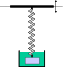
\includegraphics[width=.8\columnwidth]{images/spring_dashpot.pdf}}{\vfill
$x(t)=$ displacement from rest position\\
\vfill
Newton's 2$^{nd}$ Law:
\algn{ F &= ma\\
x\pp + \beta x\p +k x &= 0}\vspace*{\fill} }
\vfill
\twomini{.33}{.66}{\uline{Simple Harmonic Motion}
\includegraphics[width=\columnwidth]{images/sin_graph.pdf}

}{ 
\twomini{.5}{.5}{\uline{Underdamped Motion}

 \includegraphics[width=\columnwidth]{images/sin_exp_graph.pdf}}{ \uline{Overdamped Motion}

\includegraphics[width=\columnwidth]{images/exp_graph.pdf} }

}

}

\slide[Spring oscillators with forcing]{\vfill
\centerline{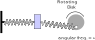
\includegraphics{images/spring_dashpot_forced.pdf}}
\vfill}

\slide[Harmonic motion with forcing]{\vspace{-1.5em}
\[x\pp+\omega_0^2 x =f(t)= \frac{F_0}{m}\cos (\omega t)\hspace{2em}\text{with}\qquad\larray{\omega\neq\omega_0\\x(0)=x\p(0)=0}\]
\student{\algn{x_h &= c_1 \cos (\omega_0 t)  +c_2 \sin (\omega_0 t)&
x_p &= A \cos (\omega t) + \cancelto{0}{B} \sin (\omega t)\\
x_p\pp&=-\omega^2A\cos (\omega t)}
\[-\omega^2A\cos (\omega t)+\omega_0^2A\cos (\omega t) = \frac{F_0}{m}\cos (\omega t)\]
\algn{-\omega^2A+\omega_0^2A &= \frac{F_0}{m} &\Rightarrow A=&\frac{F_0}{m\left(\omega_0^2-\omega^2 \right)}\\
x_p&=\frac{F_0}{m\left(\omega_0^2-\omega^2 \right)}\cos (\omega t)
}
}

}
\slide{\vspace{-1.5em}\[x\pp+\omega_0^2 x = \frac{F_0}{m}\cos (\omega t)\hspace{2em}\text{with}\qquad\larray{\omega\neq\omega_0\\x(0)=x\p(0)=0}\]
$x_h= c_1 \cos (\omega_0 t)  +c_2 \sin (\omega_0 t)$ \hfill $x_p=\frac{F_0}{m\left(\omega_0^2-\omega^2 \right)}\cos (\omega t)$\vfill
\vspace{-1.5em}\student{\algn{
\intertext{Initial Conditions:}
x(0)=0&=c_1+\frac{F_0}{m\left(\omega_0^2-\omega^2 \right)}\\
c_1&=\frac{F_0}{m\left(\omega^2-\omega_0^2 \right)}\\
x\p(0)=0&=c_2\\
x(t)& = \frac{F_0}{m\left(\omega_0^2-\omega^2 \right)} \underbrace{\left( \cos(\omega t) - \cos (\omega_0 t)  \right)}_{\carray{\sin\left( \frac{\omega_0+\omega}{2}t \right) \sin\left( \frac{\omega_0-\omega}{2} t \right)}}
}
}\vfill
}

\slide[Beat phenomena]{\vspace{-1.5em}
\[ x(t) = \frac{F_0}{m\left(\omega_0^2-\omega^2 \right)} \sin\left( \frac{\omega_0+\omega}{2}t \right) \sin\left( \frac{\omega_0-\omega}{2} t \right) \]
\vspace{.25em}
\twomini[.65]{.4}{.6}{
\tikzplot[\xcoord{1.75}{\omega_0}]{.1}{3.5}{0.1}{4}{\omega}{Amplitude}{
\draw[domain=0:1.74, samples=100, red] plot (\x, {1/(1.75*1.75-\x*\x)});
\draw[domain=1.76:3.5, samples=100, red] plot (\x, {-1/(1.75*1.75-\x*\x)});
}
}{
\tikzplot[.3]{.1}{6.5}{2}{2}{t}{x(t)}{
\draw[domain=0:10, samples=100, red] plot (\x, {sin(8000*0.01*\x)});
\draw[domain=0:10, samples=100, red] plot (\x, {-sin(8000*0.01*\x)});
\draw[domain=0:10, samples=450] plot (\x, {sin(8000*0.2*\x)*sin(8000*0.01*\x)});
\draw[|-|] (1.125,1.125) -- (3.375,1.125) node[midway, above]{$T_{beat}=\frac{4\pi}{|\omega-\omega_0|}$};
\draw[|-|] (3.2,-1.125) -- (3.4,-1.125) node[midway, below]{$T_{avg}=\frac{4\pi}{|\omega+\omega_0|}$};
}}\vfill
\centerline{What happens to $x(t)$ as $\omega\to\omega_0$?}
}

\slide[Resonance ($\omega\to\omega_0$)]{\vspace{-1.5em}
\[x\pp+\omega_0^2 x =f(t)= \frac{F_0}{m}\cos (\omega_0 t)\]

$x_h= c_1 \cos (\omega_0 t)  +c_2 \sin (\omega_0 t)$ \hspace{2em} $y_p=?$\student{\algn{y_p&\neq A \cos (\omega_0 t)  + B \sin (\omega_0 t)\\ y_p&= \cancelto{0}{A} t\cos (\omega_0 t)  + Bt \sin (\omega_0 t) & B=\frac{F_0}{2m\omega_0} }}

\twomini[.65]{.6}{.4}{
\tikzplot[.3]{.1}{6.5}{1.75}{1.75}{t}{x(t)}{
\draw[domain=0:10, samples=100, red] plot (\x, {0.25*\x)});
\draw[domain=0:10, samples=100, red] plot (\x, {-0.25*\x)});
\draw[domain=0:10, samples=450] plot (\x, {0.25*\x*sin(8000*0.1*\x)});

}
}{
As $t\to\infty$\\
\student{\centerline{Amplitude $\to\infty$}\\~\\
\centerline{Finite input power}\\~\\
\centerline{Very large response}\\~\\
\centerline{Physical Resonance}}
}
}

\slide[Damped oscillator with forcing]{
\[mx\pp+\beta x\p+kx=F_0\cos(\omega t)\]
$x(t)=x_h(t)+x_p(t)$
\vfill\student{Three cases:}
\[x_{h}(t)=\begin{cases}
e^{-\frac{\beta}{2m}t}\left(c_{1}\cos\left(\omega_{1}t\right)+c_{2}\sin\left(\omega_{1}t\right)\right) & \beta^{2}<4km\\
c_{1}e^{r_{1}t}+c_{2}e^{r_{2}t} & \beta^{2}>4km\\
c_{1}e^{rt}+c_{2}te^{rt} & \beta^{2}=4km
\end{cases}\]\vfill
\student{All exponents are negative\\\centerline{$\Rightarrow \quad x_h \to 0$ as $t\to\infty$ }}
}


\slide[Damped oscillator with forcing]{
\[mx\pp+\beta x\p+kx=F_0\cos(\omega t)\]
$x(t)=x_h(t)+x_p(t)$
\vfill
From the Method of Undetermined Coefficients:
\[x_p = A \cos (\omega t)+B \sin (\omega t)\]\vfill
As $t\to\infty$\\ \centerline{\student{$x(t) \to x_p(t)$}}\vfill
}

\slide{

\tikzplot{.1}{11}{1}{1}{t}{x_h(t)}{
\draw[domain=0:11, samples=300, smooth, Dandelion, thick] plot (\x, {  0.3*exp(-0.05*10*\x)*(-2.1611*cos(686.954*1.19896*\x) - 0.499779*sin(686.954*1.19896*\x))     });
}
\vfill
\tikzplot{.1}{11}{1}{1}{t}{x_p(t)}{
\draw[domain=0:11, samples=400, smooth, lblue, thick] plot (\x, {  0.3*(2.1611*cos(686.954*\x) + 0.491159*sin(686.954*\x))     });
}
\vfill
\tikzplot{.1}{11}{1.65}{1}{t}{x(t)}{
%\draw[domain=0:11, samples=500, Dandelion] plot (\x, {  0.3*exp(-0.05*10*\x)*(-2.1611*cos(686.954*1.19896*\x) - 0.499779*sin(686.954*1.19896*\x))     });
%\draw[domain=0:11, samples=500, lblue] plot (\x, {  0.3*(2.1611*cos(686.954*\x) + 0.491159*sin(686.954*\x))     });
\draw[domain=0:11, samples=400, smooth,  black, thick] plot (\x, {  0.3*(2.1611*cos(686.954*\x) - 2.1611*exp(-0.05*10*\x)*cos(686.954*1.19896*\x) + 0.491159*sin(686.954*\x) - 
 0.499779*exp(-0.05*10*\x)*sin(686.954*1.19896*\x))     });
\draw[|-|] (0.1,-1.125) -- (6,-1.125) node[midway, below]{transient response};
\draw[|->] (6.1,-1.125) -- (11,-1.125) node[midway, below]{steady state response};
}

}

\slide{\[mx\pp+\beta x\p+k x=\cos(\omega t)\]
How does the amplitude of the steady state response vary with $\omega$?

\student{\algn{x_p&=A\cos (\omega t) + B\sin (\omega t)\\
x_p\p &=- \omega A\sin (\omega t) + \omega B\cos (\omega t)\\
x_p\pp &=- \omega^2 A\cos (\omega t) - \omega^2 B\sin (\omega t)
}
\algn{m\left(- \omega^2 A\cos (\omega t) - \omega^2 B\sin (\omega t) \right) &+ \beta \left(  - \omega A\sin (\omega t) + \omega B\cos (\omega t) \right)\\
+ k \left( A\cos (\omega t) + B\sin (\omega t) \right) &= \cos(\omega t)\\\\
(Ak+B\beta \omega -mA\omega^2)\cos (\omega t) &+  (Bk-A\beta \omega -mB\omega^2)\sin (\omega t)  \\&= \cos (\omega t)}
}
}

\slide{
\student{Match coefficients\algn{\uline{\cos:} \qquad (Ak+B\beta \omega -mA\omega^2)&= 1\\
\uline{\sin:} \qquad  (Bk-A\beta \omega -mB\omega^2)&=0\\
B=A\frac{\beta\omega}{k-m \omega^2}&\\
 \left(Ak+A\frac{(\beta\omega)^2}{k-m \omega^2} -mA\omega^2\right)&= 1\\
A=\frac{k-m\omega^2}{(\beta\omega)^2-(k-m\omega^2)^2}&\qquad B=\frac{\beta\omega }{(\beta\omega)^2-(k-m\omega^2)^2}
}
}
}

\slide{\student{Amplitude:\algn{
R&=\sqrt{A^2+B^2}\\
&=\frac{\sqrt{(k-m\omega^2)^2 + (\beta \omega^2)}}{(\beta\omega)^2-(k-m\omega^2)^2}\\
&= \frac{1}{\sqrt{k^2 - 2 k m \omega^2 + m^2 \omega^4 + \omega^2 \beta^2}}
}
\twomini{.6}{.4}{\ucover{
\tikzplot[]{.1}{6}{.1}{4}{\omega}{}{
\draw[domain=0:11, samples=400, smooth,  black, thick] plot (\x, { 0.5/sqrt(4-3.99*\x*\x+\x*\x*\x*\x)  });
}}}{
}
}
}
\settoggle{covered}{false}

\slide[Amplitude vs Forcing Frequency]{
Steady-state response: $x_p = R \cos(\omega t-\phi)$ with
\algn{R(\omega) & =  \frac{1}{\sqrt{k^2 - 2 k m \omega^2 + m^2 \omega^4 + \omega^2 \beta^2}} \\ &= \frac{1}{\sqrt{\beta ^2 \omega ^2+\left(k-m \omega ^2\right)^2}} }
What value of $\omega$ creates the largest amplitude response?
\student{
\algn{\dd{}{\omega} R & = -\frac{\omega  \left(\beta ^2-2 k m+2 m^2 \omega ^2\right)}{\left(\beta ^2 \omega ^2+\left(k-m \omega ^2\right)^2\right)^{3/2}} =0\\\\
\text{Critical points:} \qquad \omega^* &= 0, \quad \pm \sqrt{ \frac{k}{m}- \frac12\paren{\frac{\beta}{m}} ^2}}

}

}


\slide[Amplitude vs Forcing Frequency]{
\twomini{0.55}{0.45}{
Underdamped:
\[x_h = e^{-\frac{\beta}{2m}t}(c_1\cos(\omega_1 t) + c_2\sin(\omega_1 t))\]
$\omega_1 = \sqrt{\frac{k}{m}-\paren{\frac{\beta}{2m}}^2 }$

\tikzplot[\xcoord{1.105}{\quad\; \omega_1} \xcoord{1.05}{\omega^*\quad\;}]{.1}{4}{.1}{2.5}{\omega}{}{
\draw[domain=0:4, samples=400, smooth,  black, thick] plot (\x, { 10/sqrt(64-80*\x*\x+36*\x*\x*\x*\x)  });
\draw[black, dashed] (1.05,0) -- (1.05,2.26134);
}
\[\omega^* = \sqrt{ \frac{k}{m}- \frac12\paren{\frac{\beta}{m}} ^2} \approx \omega_1\]
}{Overdamped:
\[x_h = c_1e^{r_1t} + c_2e^{r_2t}\]
$r_{1,2} = \frac{-\beta \pm \sqrt{\beta^2 -4km}}{2m}$

\tikzplot[ \xcoord{0}{\omega^*}]{.1}{4}{.1}{2.5}{\omega}{}{
\draw[domain=0:4, samples=400, smooth,  black, thick] plot (\x, { 15/sqrt(64+80*\x*\x+36*\x*\x*\x*\x)  });


}
\[\omega^*=0\]
}
}

\slide[Resonance with damped oscillators?]{
\[mx\pp+\beta x\p+ kx=\frac{F_0}{m}\cos(\omega t)\]
What happens as $\omega \to \omega^*$?

\vfill
\student{
\itmz{
\item  Transient response \subitem{amplitude and duration both grow larger}
\item Steady state response  \subitem{amplitude grows larger}
}\vfill
\centerline{This is called quasi-resonance.}
}
\vfill
}

\end{document}